\chapter{Evaluation}\label{ch:evaluation}
Das folgende Kapitel dient dem Vergleich zwischen BloomFilterTree und der bisherigen Organisation der Bloom-Filter in AMBIENCE. Abschnitt \ref{sec:datensatz} beschreibt den Datensatz, der für die Evaluation verwendet wurde. Er stammt nicht aus AMBIENCE, sondern die Bloom-Filter wurden wie in Abschnitt \ref{sec:umsetzung} beschrieben selbst implementiert. Der Versuchsaufbau, d.h. welche Aspekte untersucht und verglichen wurden, findet sich in Abschnitt \ref{sec:versuchsaufbau}. Die erzielten Ergebnisse werden in Abschnitt \ref{sec:ergebnisse} vorgestellt und in Abschnitt \ref{sec:interpretation} ausgewertet.
\section{Datensatz}\label{sec:datensatz}
Obgleich nicht mit echten AMBIENCE-Daten gearbeitet wurde, wurde versucht ein möglichst realistisches Szenario zu erstellen. Folgende Parameter wurden verwendet:
\begin{center}
\begin{table}[htbp]
{\small
\begin{center}
\begin{tabular}[center]{lcc}
\toprule
\textbf{Filtergröße} & 256 Bit & 512 Bit\\
\midrule
\textbf{Anzahl Bloom-Filter (\textit{m})} & 100 & 100\\
\midrule
\textbf{Anzahl eingefügte Objekte (\textit{n})} & 50 & 50\\
\midrule
\textbf{Anzahl Hashfunktionen (\textit{d})} & 4 & 8\\
\bottomrule
\end{tabular}
\end{center}
} % end of tiny
\caption[Datensatz für den Versuchsaufbau]{Datensatz für den Versuchsaufbau.\label{tab:Datensatz}}
\end{table}
\end{center}
Als Wörterbuch wurde die Unix-Datei \texttt{words} verwendet\footnote{Sie befindet sich auf Unix- und Unix-ähnlichen Systemen normalerweise unter \texttt{/usr/share/dict/words} oder \texttt{/usr/dict/words}.}. Daraus wurden jeweils 50 zufällig gewählte Einträge in die Bloom-Filter eingefügt. Dazu wurden wie in Abschnitt \ref{sec:hashfunktionen} erläutert Murmur-Hashfunktionen verwendet. Die Anzahl der zu verwendenden Hashfunktionen lässt sich berechnen als 
\[d = \Ceil[\Bigg]{\frac{m}{n} * ln(2)}.\]
\noindent
Der \textit{i+1}-te Hashwert wurde dabei jeweils aus dem \textit{i}-ten Hashwert berechnet wie in Abschnitt \ref{sec:bloom-implementierung} beschrieben. Den Bloom-Filtern wurden zunächst zufällige IDs zugewiesen. Sie wurden jeweils in einen BloomFilterTree und in einen Bloom-Filter-Vektor\footnote{Objekte vom Typ \texttt{std::vector<BloomFilter>}.} eingefügt, der die unsortierte Liste repräsentiert.
\newpage
\section{Versuchsaufbau}\label{sec:versuchsaufbau}
Der Versuchsaufbau vergleicht die Indexstruktur BloomFilterTree mit einer unsortierten Liste von Bloom-Filtern an Hand von ausgewählten Aspekten. Für beide Filtergrößen wurden fünf Experimente durchgeführt:  
\begin{enumerate}
	\item Ergebnisqualität
	\item CPU-Zeit 
	\item Speicherbedarf 
	\item Komplexität 
	\item Aufbaukosten 
\end{enumerate}
\paragraph*{Ergebnisqualität}
Zur Ermittlung der Ergebnisqualität wurde eine nächste-Nachbarn-Suche und eine 3-nächste-Nachbarn-Suche auf dem BloomFilterTree durchgeführt. Die erzielten Ergebnisse wurden mit den Sollwerten einer regulären \textit{k}-nächste-Nachbarn-Suche verglichen. 
\paragraph*{CPU-Zeit}
Zur Messung der CPU-Zeit wurde die C++-Bibliothek \texttt{chrono} verwendet. Es wurden jeweils die Ausführungszeiten der Funktionen \texttt{simQuery()} und \texttt{simQueryVec()} für $k=1$ bzw. $k=3$ (vgl. Abschnitt \ref{sec:knn}) ermittelt und mit den Ausführungszeiten einer regulären \textit{k}-nächste-Nachbarn-Suche verglichen.
\paragraph*{Speicherbedarf} 
Da der BloomFilterTree nur Zeiger auf Bloom-Filter-Objekte enthält und nicht die Datenstrukturen selbst, ist sein Speicherbedarf eher gering. %TODO Angabe 
Zur Ermittlung des Speicherbedarfs wurde daher von den tatsächlich allokierten Instanzen der Klasse \texttt{BloomFilter} ausgegangen. Das sind bei einer unsortierten Liste alle eingefügten Bloom-Filter, beim BloomFilterTree zusätzlich die Vereinigungsfilter aller Knoten. Diese Speicherbedarfe wurden für BloomFilterTree und unsortierte Liste ermittelt und gegenüber gestellt. 
\paragraph*{Komplexität}
Zur Ermittlung der Komplexität der unterschiedlichen Suchalgorithmen wurde die Anzahl Vergleiche, die zur Anfragebeantwortung notwendig sind, als Maß verwendet. Diese wurden für BloomFilterTree und unsortierte Liste ermittelt und verglichen. Für den BloomFilterTree wurden dazu Varianten der Funktionen \texttt{simQuery()} und \texttt{simQueryVec()} implementiert, die die Anzahl an durchgeführten Vergleichen exakt mitprotokollieren.   
\paragraph*{Aufbaukosten}
Als Maß für die Aufbaukosten von BloomFilterTree und unsortierter Liste wurde die Zeitkomplexität des Einfügens aller Elemente verwendet. Diese liegt für Objekte vom Typ \texttt{std::vector} mit \textit{n} Elementen durchschnittlich in $O(1)$ für die verwendete Funktion \texttt{std::vector::push\_back()}\footnote{Vgl. \url{http://www.cplusplus.com/reference/vector/vector/push_back/.}}. 

Beim BloomFilterTree setzt sich die Komplexität der Einfüge-Operation aus der Berechnung der optimalen Teilmengen- und Obermengen-IDs und dem tatsächlichen Einfügen des Objekts zusammen. Wie in Abschnitt \ref{sec:einfügen} dargestellt ist die Berechnung der Teilmengen-IDs aufwändig und macht die Einfüge-Operation deutlich teurer als das kanonische Einfügen im B$^+$-Baum. Die Operationen mit der größten Zeitkomplexität sind hierbei das Sortieren der freien und "`guten"' IDs. Die Kosten für den Aufbau der Indexstruktur liegen damit insgesamt in $O(n\ast log(n))$ für einen BloomFilterTree mit \textit{n} Elementen. 
\section{Ergebnisse}\label{sec:ergebnisse}
Im Folgenden werden die Ergebnisse der fünf Experimente mit den beschriebenen Parametern vorgestellt. 
\paragraph*{Ergebnisqualität}
Abbildungen \ref{fig:pic8} und \ref{fig:pic9} stellen die Ergebnisqualität der nächste-Nachbarn-Suche dar. Die Sollwerte sind darin grün, die Messwerte blau markiert. Stimmt der Messwert mit dem Sollwert überein, ist nur die blaue Markierung vorhanden. Der quadratische Fehler von Messwert gegenüber Sollwert ist in Rot angegeben. 
\begin{figure}[hpbt]
	\centering
 	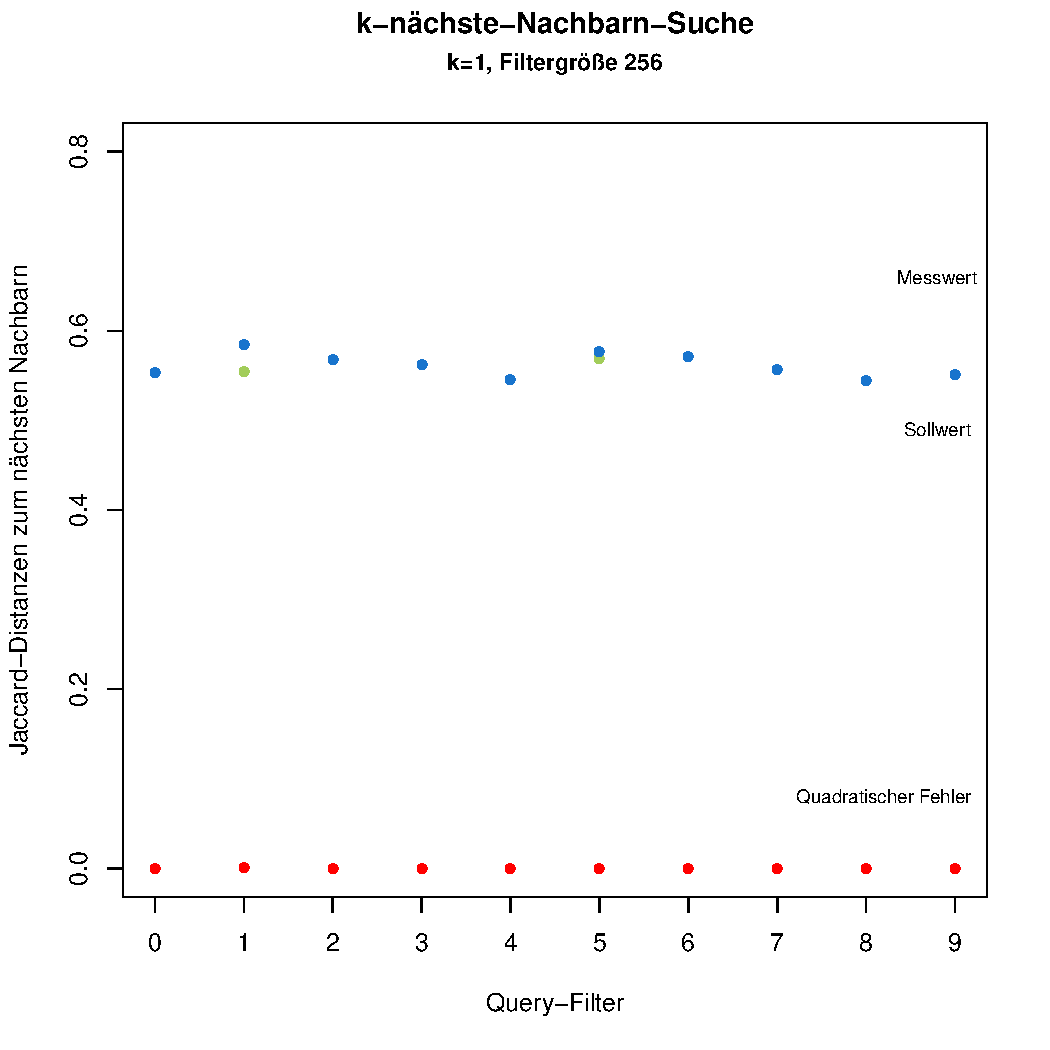
\includegraphics[scale=0.7]{pictures/nn_256.pdf}\\
  	\caption[Ergebnisqualität der nächste-Nachbarn-Suche für 256 Bit-Bloom-Filter]{Ergebnisqualität der nächste-Nachbarn-Suche für 256 Bit-Bloom-Filter.}\label{fig:pic7}
 	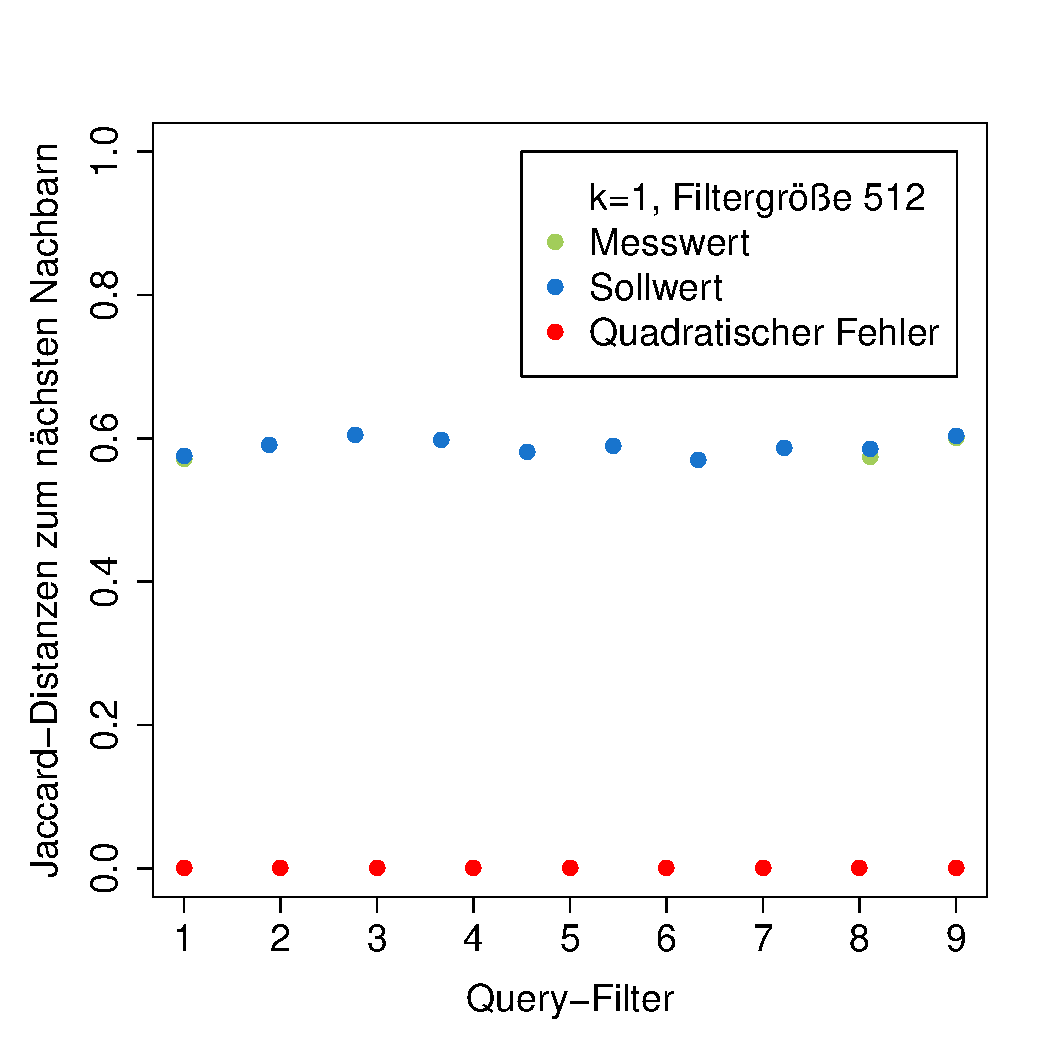
\includegraphics[scale=0.7]{pictures/nn_512.pdf}\\
  	\caption[Ergebnisqualität der nächste-Nachbarn-Suche für 256 Bit-Bloom-Filter]{Ergebnisqualität der nächste-Nachbarn-Suche für 512 Bit-Bloom-Filter.}\label{fig:pic8}
\end{figure}

Abbildungen \ref{fig:pic9} -- \ref{fig:pic12} stellen die Ergebnisqualität der 3-nächste-Nachbarn-Suche dar. Die Sollwerte sind darin in drei Grünstufen markiert, die Messwerte sind in drei Blaustufen markiert. Der mittlere quadratische Fehler der Messwerte gegenüber den Sollwerten ist in Rot angegeben.
\begin{figure}
	\centering
	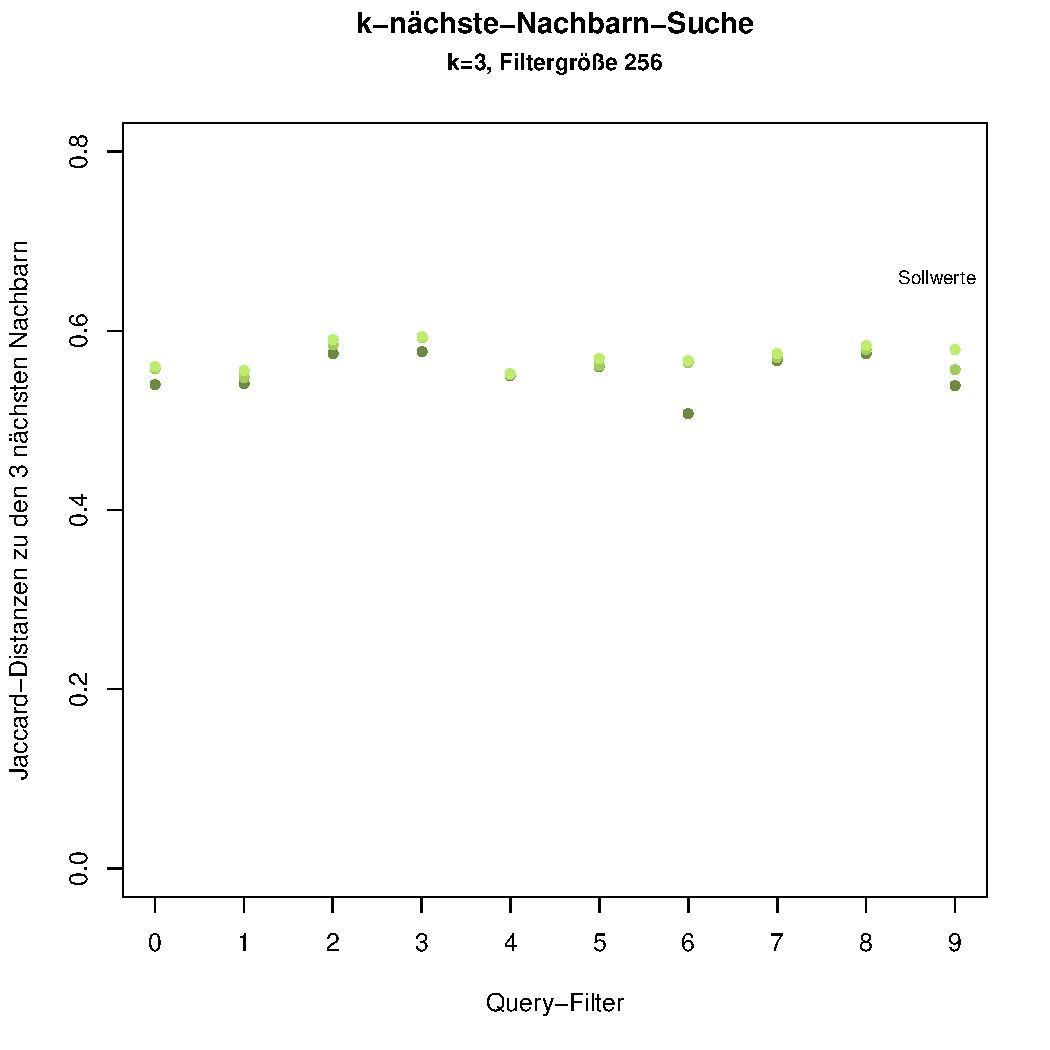
\includegraphics[scale=0.7]{pictures/nn3_256-1.pdf}\\
	\caption[Sollwerte der 3-nächste-Nachbarn-Suche für 256 Bit-Bloom-Filter]{Sollwerte der 3-nächste-Nachbarn-Suche für 256 Bit-Bloom-Filter.}\label{fig:pic9}
	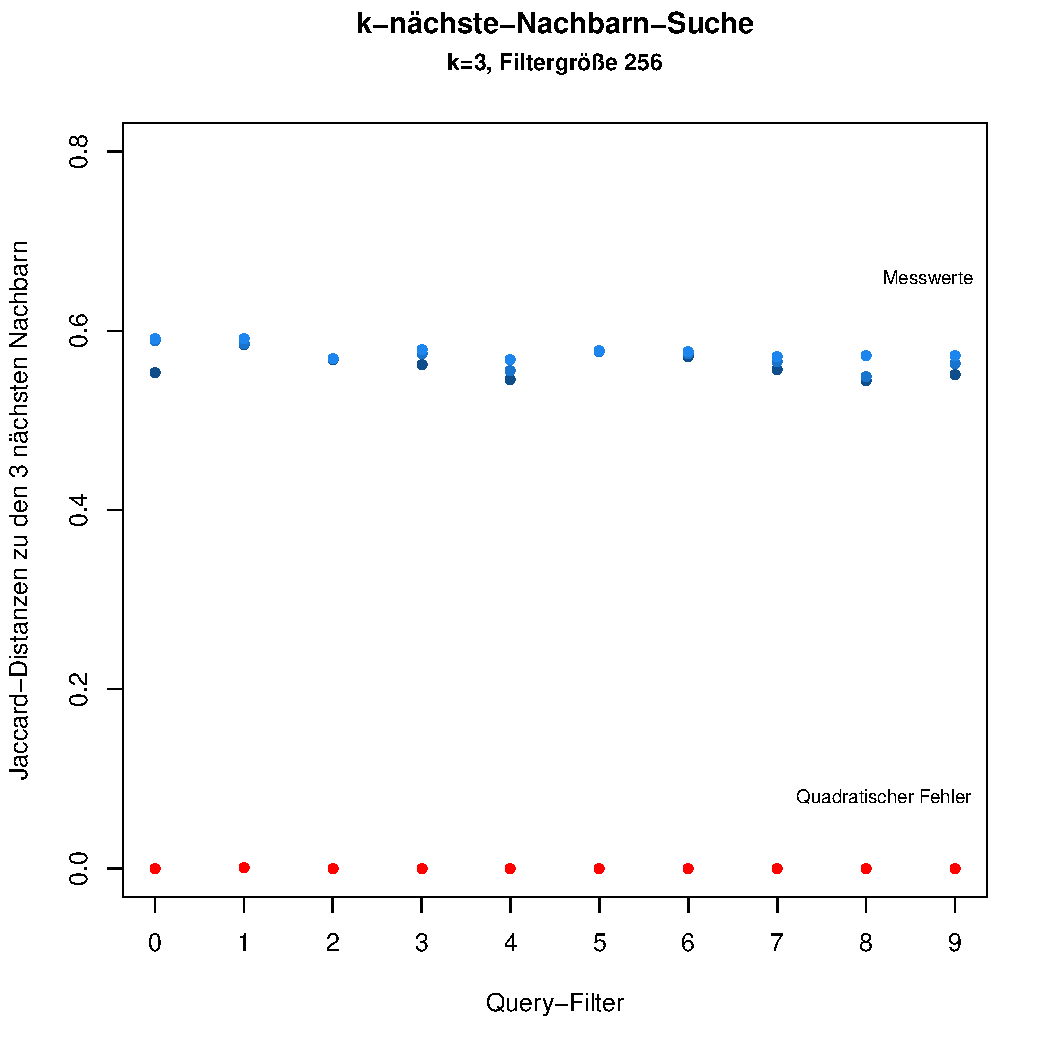
\includegraphics[scale=0.7]{pictures/nn3_256-2.pdf}\\
	\caption[Messwerte der 3-nächste-Nachbarn-Suche für 512 Bit-Bloom-Filter]{Messwerte der 3-nächste-Nachbarn-Suche für 512 Bit-Bloom-Filter.}\label{fig:pic10}
\end{figure}
\begin{figure}[hptb]
	\centering
	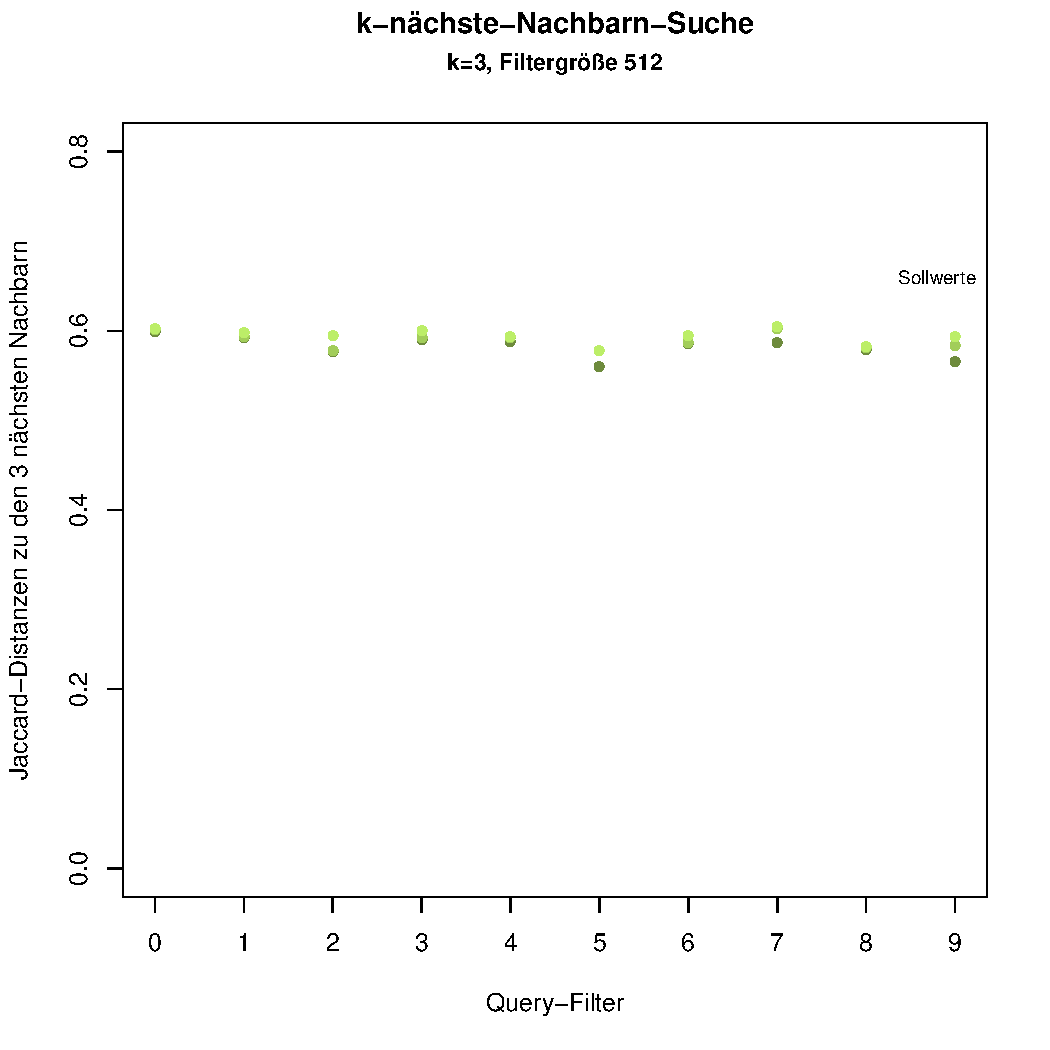
\includegraphics[scale=0.7]{pictures/nn3_512-1.pdf}\\
	\caption[Sollwerte der 3-nächste-Nachbarn-Suche für 512 Bit-Bloom-Filter]{Sollwerte der 3-nächste-Nachbarn-Suche für 512 Bit-Bloom-Filter.}\label{fig:pic11}
	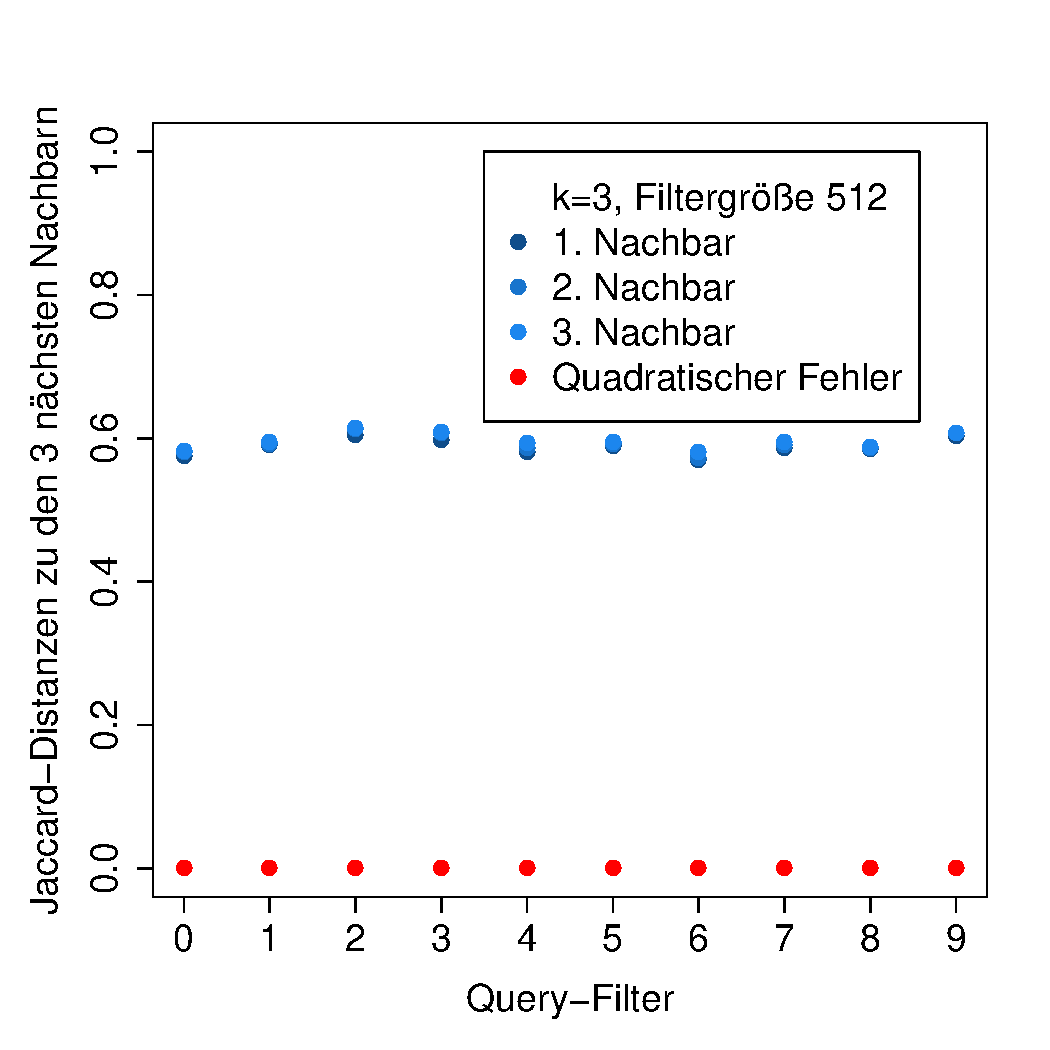
\includegraphics[scale=0.7]{pictures/nn3_512-2.pdf}\\
	\caption[Messwerte der 3-nächste-Nachbarn-Suche für 512 Bit-Bloom-Filter]{Messwerte der 3-nächste-Nachbarn-Suche für 512 Bit-Bloom-Filter.}\label{fig:pic12}
\end{figure}
\paragraph*{CPU-Zeit}
Abbildungen \ref{fig:pic13} und \ref{fig:pic14} stellen die CPU-Zeit zur Ausführung der nächste-Nachbarn-Suche dar. Die Ergebnisse für den BloomFilterTree sind darin blau, die Ergebnisse für die unsortierte Liste grün markiert.  
\begin{figure}[hptb]
	\centering
	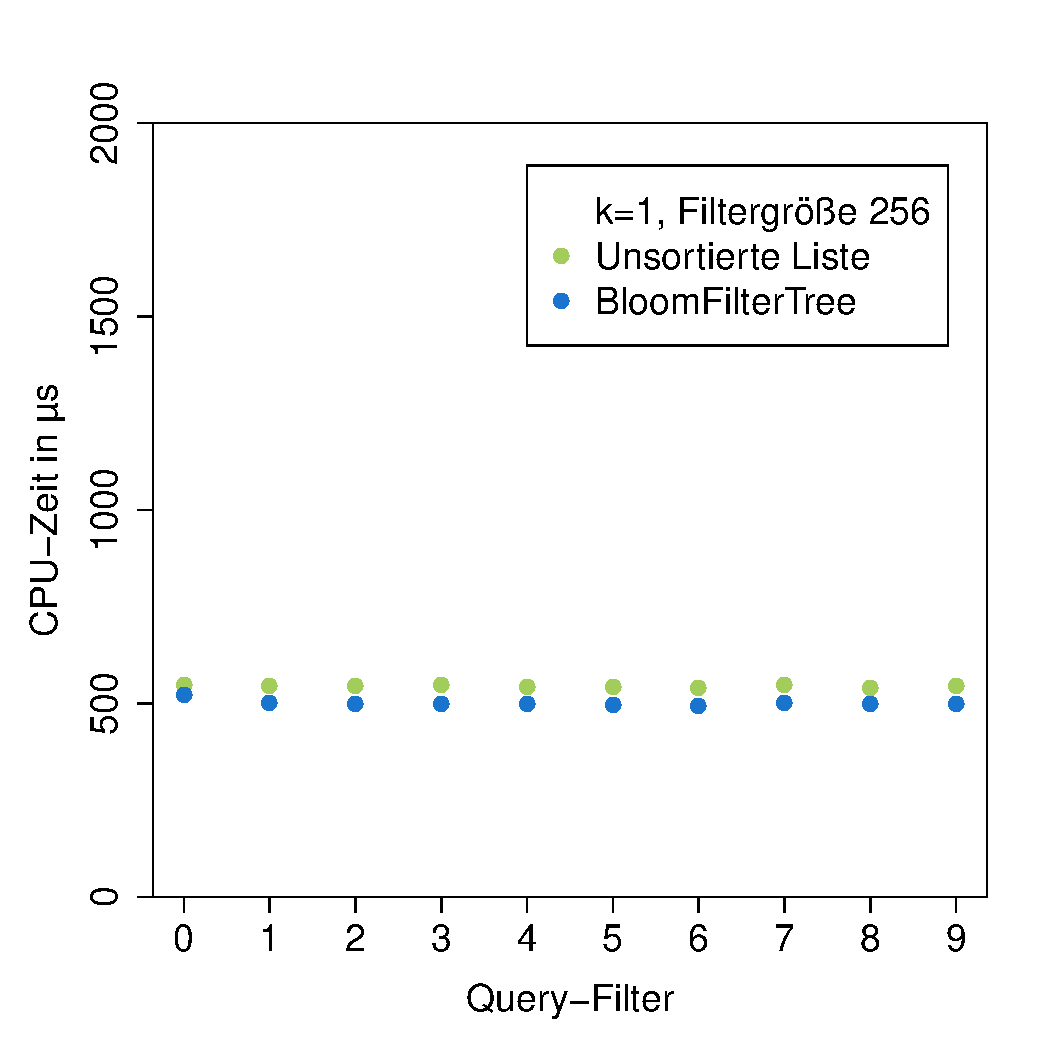
\includegraphics[scale=0.7]{pictures/cputime_nn_256.pdf}\\
	\caption[CPU-Zeit für nächste-Nachbarn-Suche mit 256 Bit-Bloom-Filtern]{CPU-Zeit für \textit{k}-nächste-Nachbarn-Suche mit 256 Bit-Bloom-Filtern.}\label{fig:pic13}
	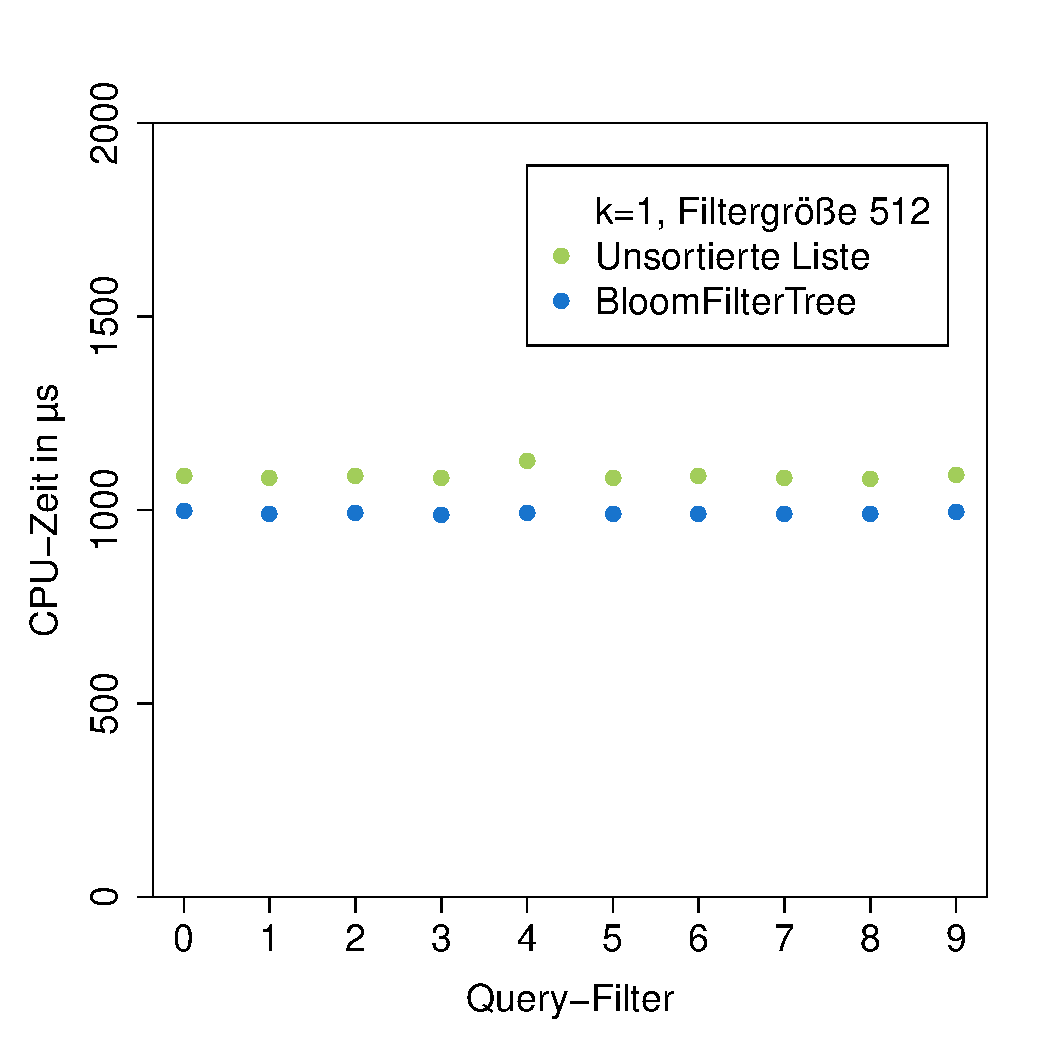
\includegraphics[scale=0.7]{pictures/cputime_nn_512.pdf}\\
	\caption[CPU-Zeit für nächste-Nachbarn-Suche mit 512 Bit-Bloom-Filtern]{CPU-Zeit für \textit{k}-nächste-Nachbarn-Suche mit 512 Bit-Bloom-Filtern.}\label{fig:pic14}
\end{figure}

Abbildungen \ref{fig:pic15} und \ref{fig:pic16} stellen die CPU-Zeit zur Ausführung der 3-nächste-Nachbarn-Suche dar. Die Ergebnisse für den BloomFilterTree sind darin blau, die Ergebnisse für die unsortierte Liste grün markiert.  
\begin{figure}[hptb]
	\centering
	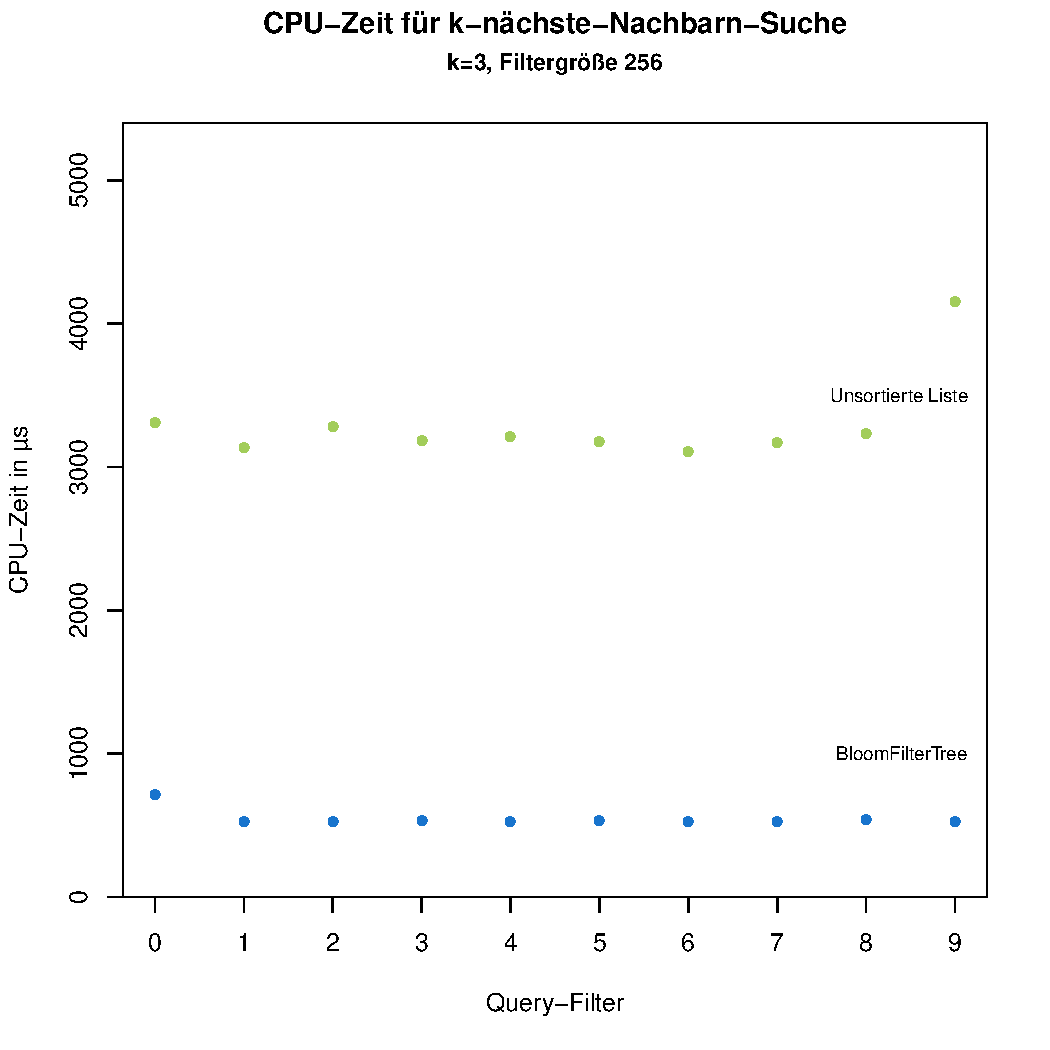
\includegraphics[scale=0.7]{pictures/cputime_nn3_256.pdf}\\
	\caption[CPU-Zeit für 3-nächste-Nachbarn-Suche mit 256 Bit-Bloom-Filtern]{CPU-Zeit für nächste-Nachbarn-Suche mit 256 Bit-Bloom-Filtern.}\label{fig:pic15}
	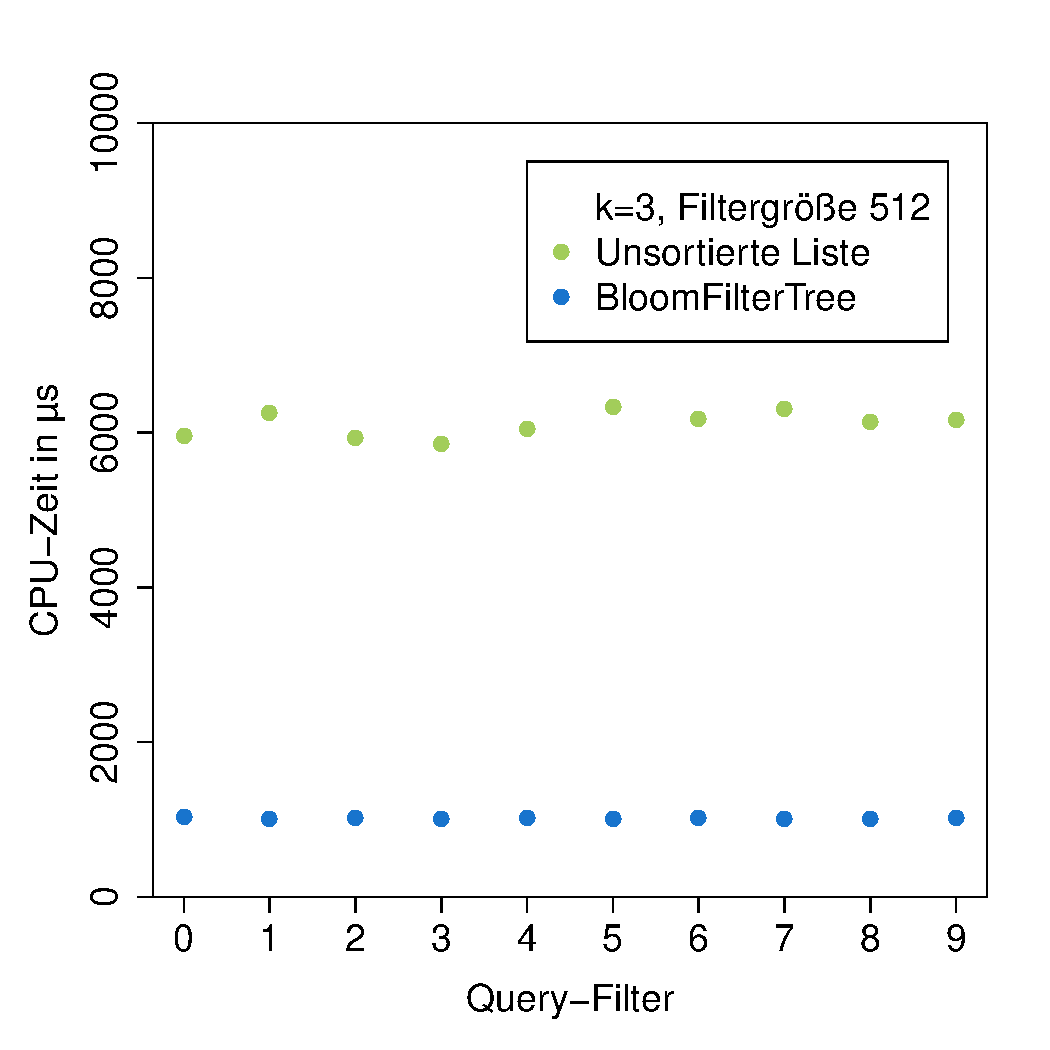
\includegraphics[scale=0.7]{pictures/cputime_nn3_512.pdf}\\
	\caption[CPU-Zeit für 3-nächste-Nachbarn-Suche mit 512 Bit-Bloom-Filtern]{CPU-Zeit für nächste-Nachbarn-Suche mit 512 Bit-Bloom-Filtern.}\label{fig:pic16}
\end{figure}
\paragraph*{Speicherbedarf}
Abbildung \ref{fig:pic17} stellt den Speicherbedarf für BloomFilterTree und unsortierte Liste gegenüber. Objekte vom Typ BloomFilterTree sind darin blau, Objekte vom Typ \texttt{std::vector<BloomFilter>} grün markiert. 
\begin{figure}[hptb]
	\centering
	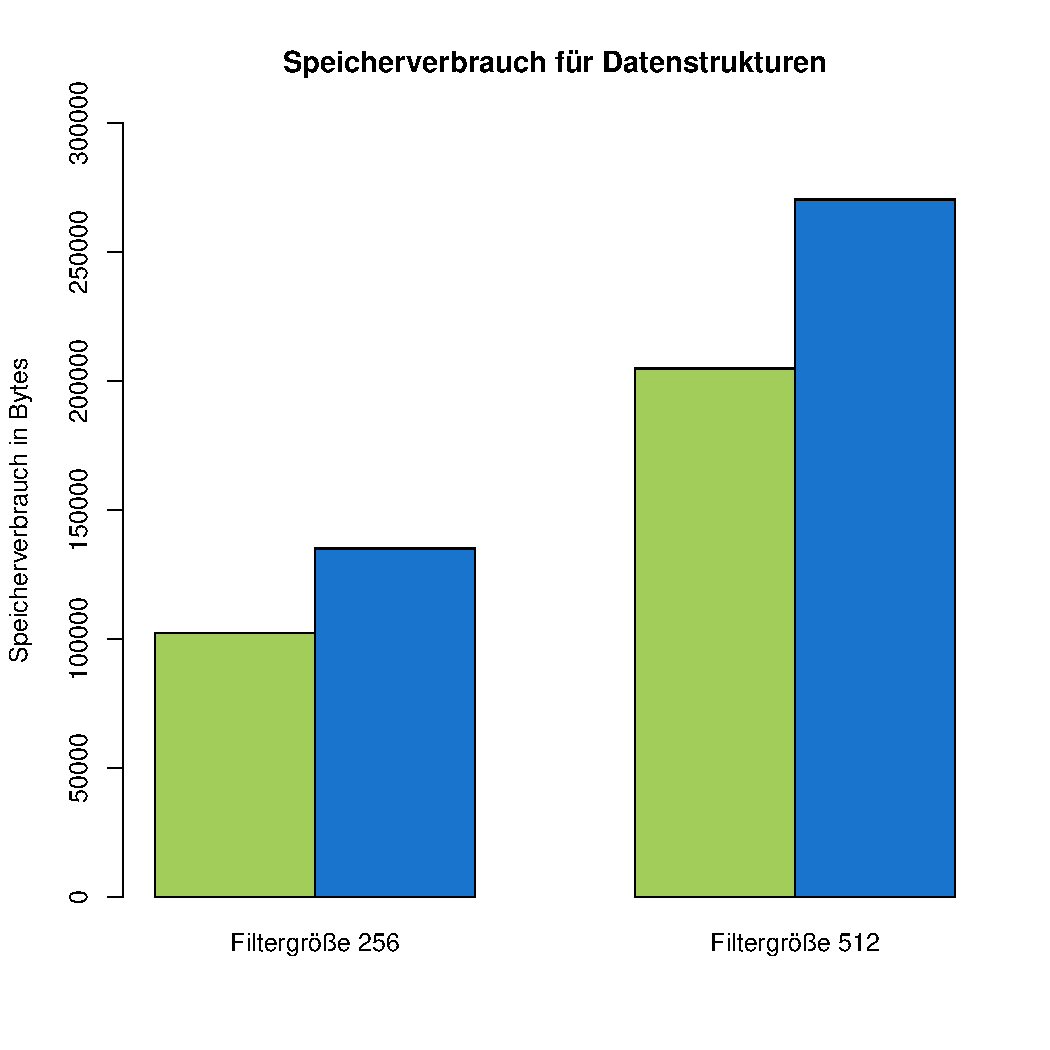
\includegraphics[scale=0.7]{pictures/mem.pdf}\\
	\caption[Speicherbedarf für BloomFilterTree und unsortierte Liste]{Speicherbedarf für BloomFilterTree und unsortierte Liste.}\label{fig:pic17} 
\end{figure}	
\paragraph*{Komplexität}
Abbildung \ref{fig:pic18} stellt die Komplexität der \textit{k}-nächste-Nachbarn-Suche wie in Abschnitt \ref{sec:versuchsaufbau} beschrieben als Anzahl von Vergleichen dar, die zur Anfragebearbeitung nötig sind. Die Ergebnisse sind darin für den BloomFilterTree blau, für die unsortierte Liste grün markiert.
\begin{figure}[hptb]
	\centering
	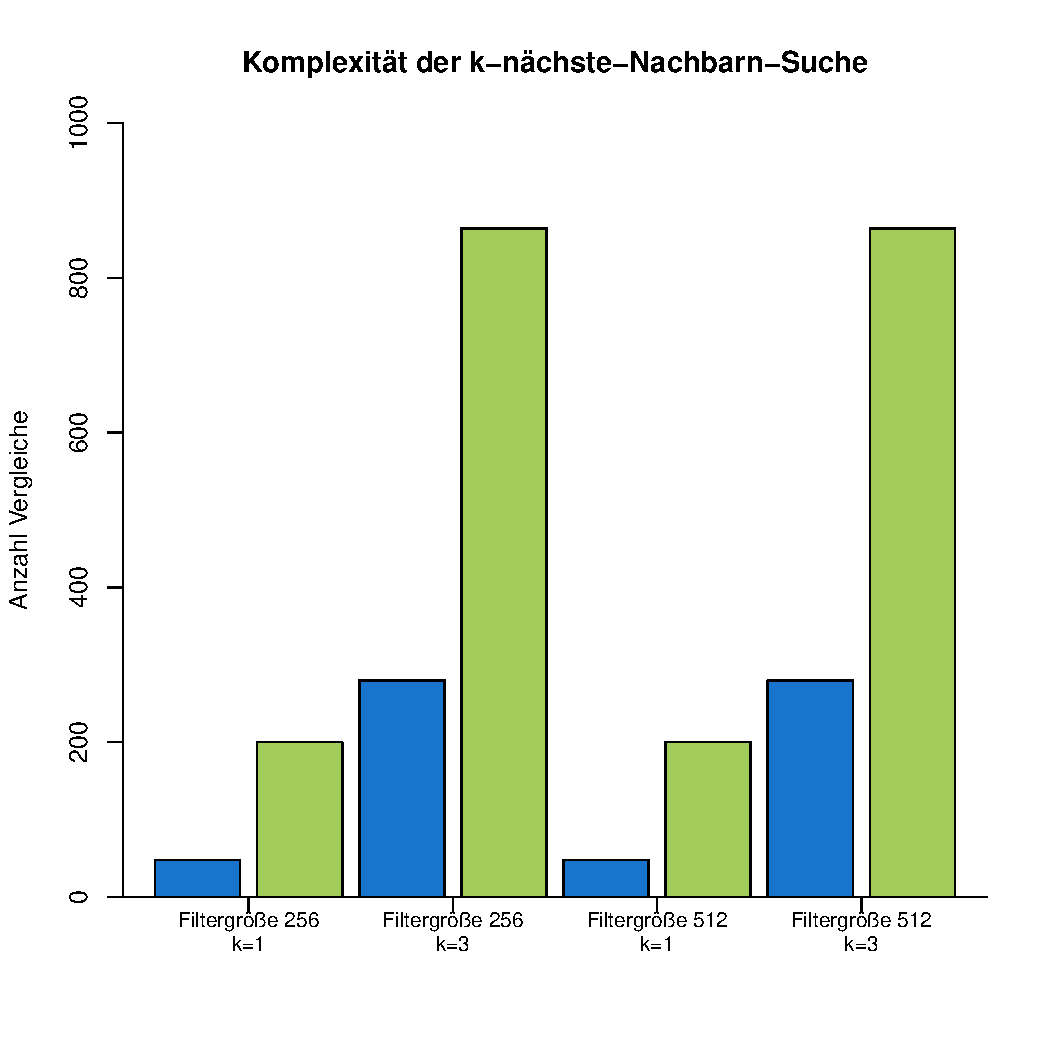
\includegraphics[scale=0.7]{pictures/compl.pdf}\\
	\caption[Komplexität der \textit{k}-nächste-Nachbarn-Suche auf BloomFilterTree und unsortierter Liste]{Komplexität der \textit{k}-nächste-Nachbarn-Suche auf BloomFilterTree und unsortierter Liste.}\label{fig:pic18}
\end{figure} 
\paragraph*{Aufbaukosten}
Abbildung \ref{fig:pic19} stellt die Aufbaukosten der angelegten Objekte dar. Die Aufbaukosten für Objekte vom Typ BloomFilterTree sind darin blau markiert. Die Aufbaukosten für Objekte vom Typ \texttt{std::vector<BloomFilter>} sind grün markiert. 
\begin{figure}[hptb]
	\centering
	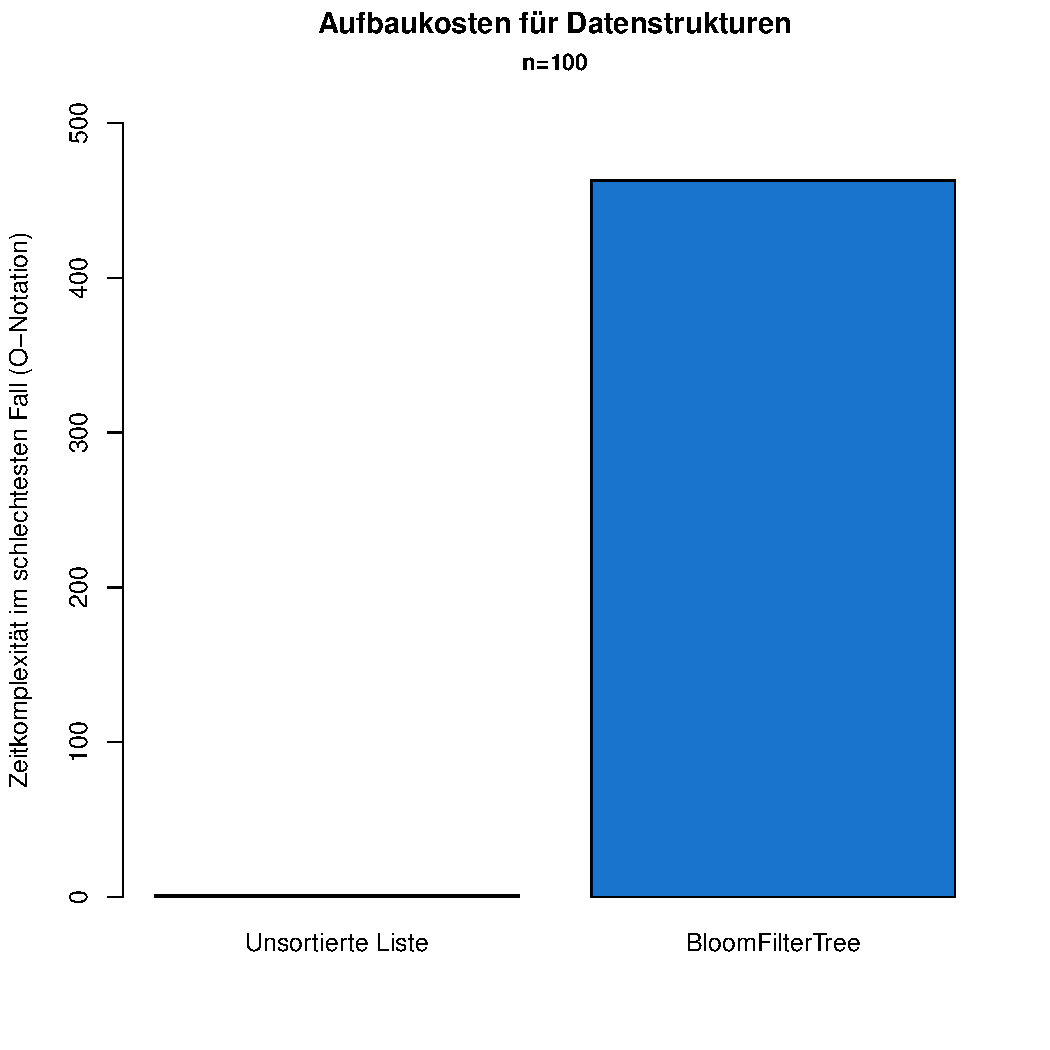
\includegraphics[scale=0.7]{pictures/cost.pdf}\\
	\caption[Aufbaukosten für BloomFilterTree und unsortierte Liste]{Aufbaukosten für BloomFilterTree und unsortierte Liste.}\label{fig:pic19}
\end{figure}
\newpage
\section{Interpretation}\label{sec:interpretation}
Wie in Abschnitt \ref{sec:datensatz} dargestellt, wurde die Evaluation mit zehn Anfragefiltern pro Experiment durchgeführt. Die Ergebnisse sind also dazu geeignet, etwaige Ausreißer zu erkennen. Das gilt insbesondere für die Ergebnisse der CPU-Zeitmessung, die in der Regel wegen schwankender Nutzlast der verwendeten Maschine und nicht exakt vorhersehbaren CPU-Schedulings gewissen Schwankungen unterliegen. Demnach kann hierbei das Minimum der erzielten Messwerte als Benchmark angesehen werden. 
\paragraph*{Ergebnisqualität}
Die Ergebnisse der \textit{k}-nächste-Nachbarn-Suche stimmen zum größten Teil mit den Sollwerten überein. Bei der nächsten-Nachbarn-Suche mit 256 Bit-Bloom-Filtern treten zwei abweichende Ergebnisse auf (vgl. Abbildung \ref{fig:pic7}). Bei der 3-nächste-Nachbarn-Suche mit 256-Bit-Filtern treten bei 30 Ergebnissen fünf abweichende Einzelergebnisse auf. Bei der 3-nächste-Nachbarn-Suche mit 512-Bit-Filtern treten bei 30 Ergebnissen sechs abweichende Einzelergebnisse auf. 

Der quadratische Fehler für diese Fälle beträgt bei der nächste-Nachbarn-Suche mit 256 Bit-Bloom-Filtern maximal 0.0008548022, andernfalls 0. Bei der 3-nächste-Nachbarn-Suche mit 256 Bit-Bloom-Filtern beträgt der mittlere quadratische Fehler bei abweichenden Messwerten maximal 0.0002956207, andernfalls 0. Bei der 3-nächste-Nachbarn-Suche mit 512 Bit-Bloom-Filtern beträgt er maximal 0.00008640455, andernfalls 0.

Das bedeutet: Nächste-Nachbarn-Anfragen werden mit dem entwickelten Verfahren in den meisten Fällen korrekt beantwortet. In wenigen Fällen werden suboptimale Antworten zurückgegeben. Diese sind dennoch als relativ "`gute"' Antworten bezüglich des verwendeten Datensatzes und des quadratischen Fehlers zu bezeichnen. Dieses Resultat ist essentiell für die Bewertung des entwickelten Verfahrens. Es kann nur dann zuverlässig eingesetzt werden, wenn es in einem Großteil der Fälle zufriedenstellende Ergebnisse bzw. optimale Antworten liefert. 
\paragraph*{CPU-Zeit}
Die drastisch reduzierte CPU-Zeit ist als entscheidender Vorteil des entwickelten Verfahrens zu betrachten. In der verwendeten Versuchsanordnung kommt sie vor allem bei der 3-nächste-Nachbarn-Suche zum Tragen. Abbildung \ref{fig:multipic1} stellt die jeweils erreichte CPU-Zeitersparnis gegenüber:
\begin{figure}[hpbt]
 \centering
  %%----start of first subfigure----
  \subfloat[CPU-Zeitersparnis für nächste-Nachbarn-Suche mit 256-Bit-Bloom-Filtern]{
   \label{fig:multipic1:a} %% label for first subfigure
   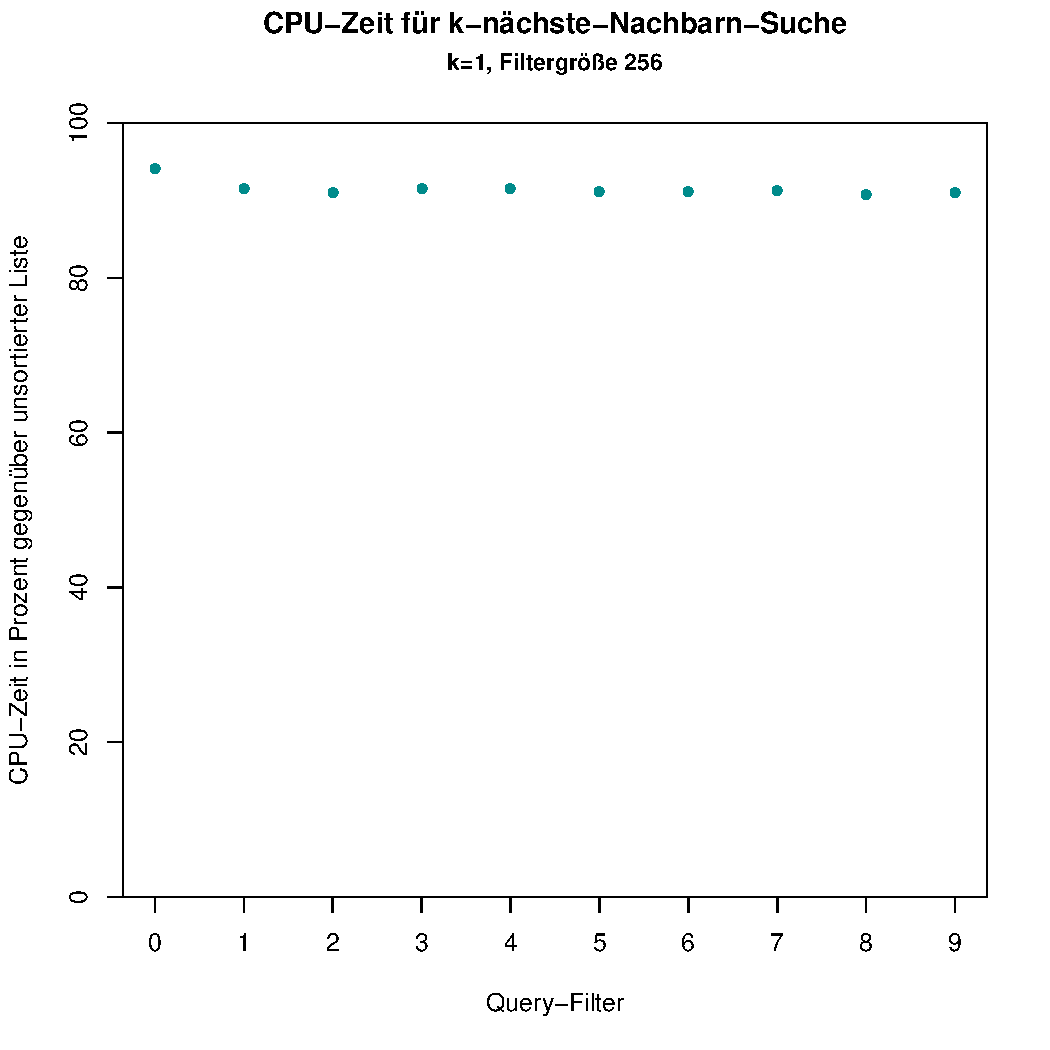
\includegraphics[width=0.48\linewidth]{pictures/percent_time_nn_256.pdf}}
  \hspace{0.01\textwidth}
  %%----start of second subfigure----
  \subfloat[CPU-Zeitersparnis für nächste-Nachbarn-Suche mit 512-Bit-Bloom-Filtern]{
   \label{fig:multipic1:b} %% label for second subfigure
   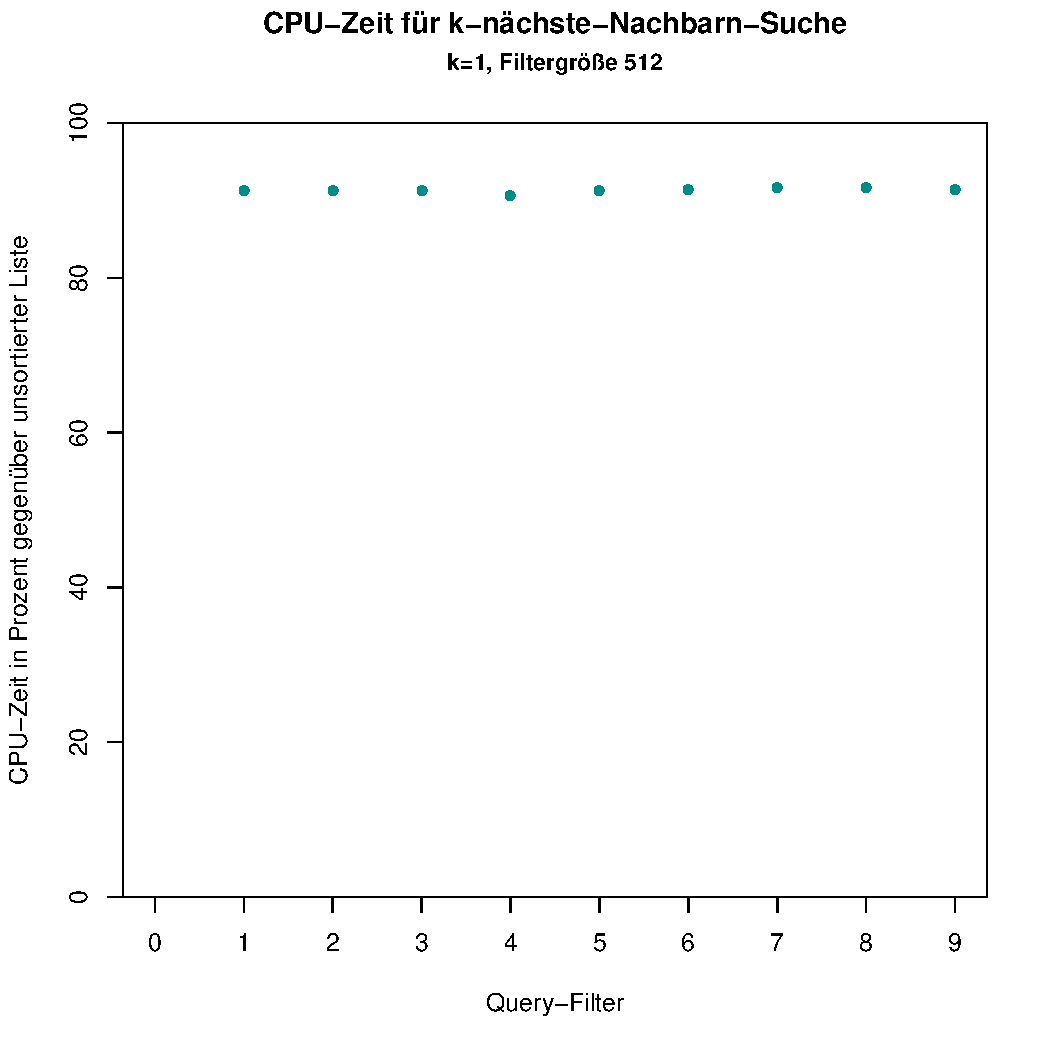
\includegraphics[width=0.48\linewidth]{percent_time_nn_512.pdf}}\\[0pt] % horizontal break
  %%----start of third subfigure----
  \subfloat[CPU-Zeitersparnis für 3-nächste-Nachbarn-Suche mit 256-Bit-Bloom-Filtern]{
   \label{fig:multipic1:c} %% label for third subfigure
   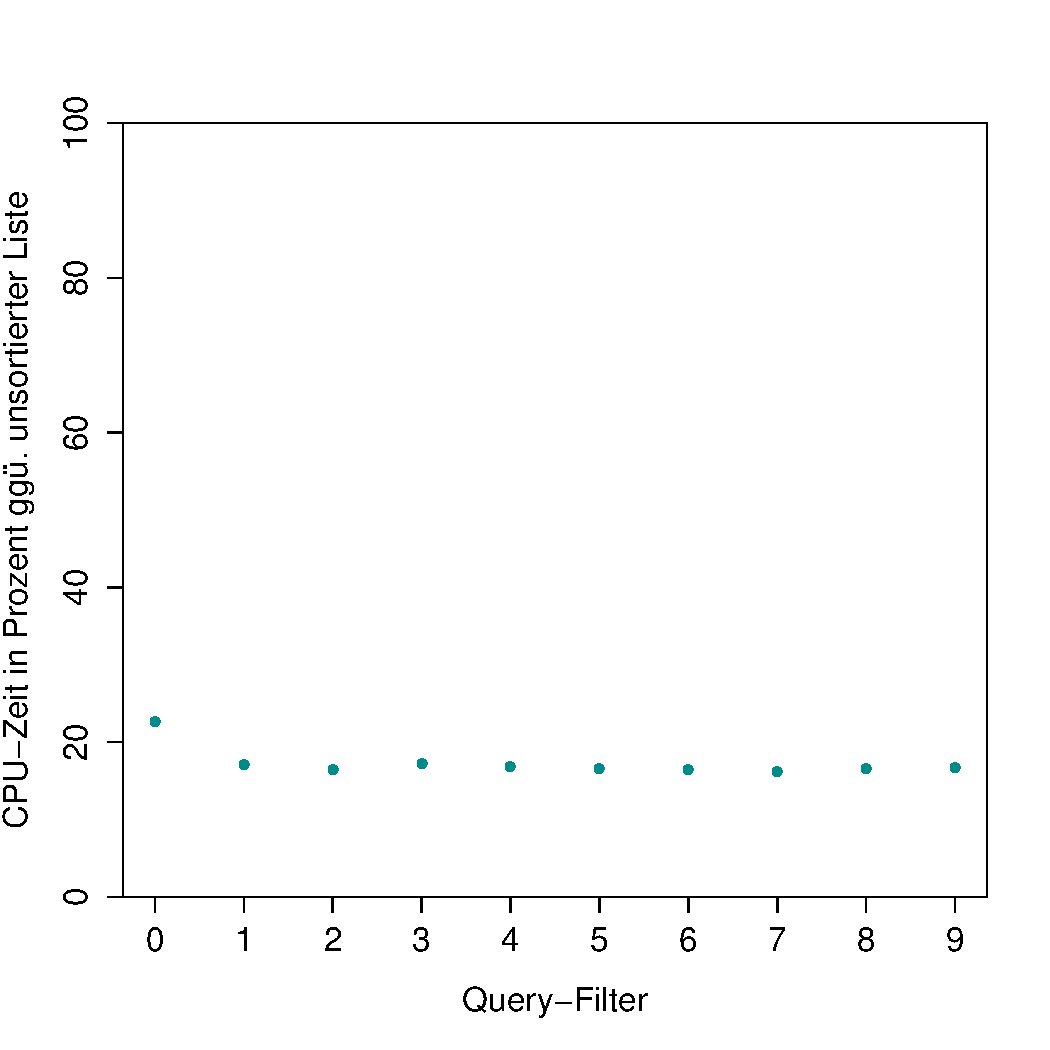
\includegraphics[width=0.48\linewidth]{pictures/percent_time_nn3_256.pdf}}
  \hspace{0.01\textwidth}
  %%----start of fourth subfigure----
  \subfloat[CPU-Zeitersparnis für 3-nächste-Nachbarn-Suche mit 512-Bit-Bloom-Filtern]{
   \label{fig:multipic1:d} %% label for fourth subfigure
   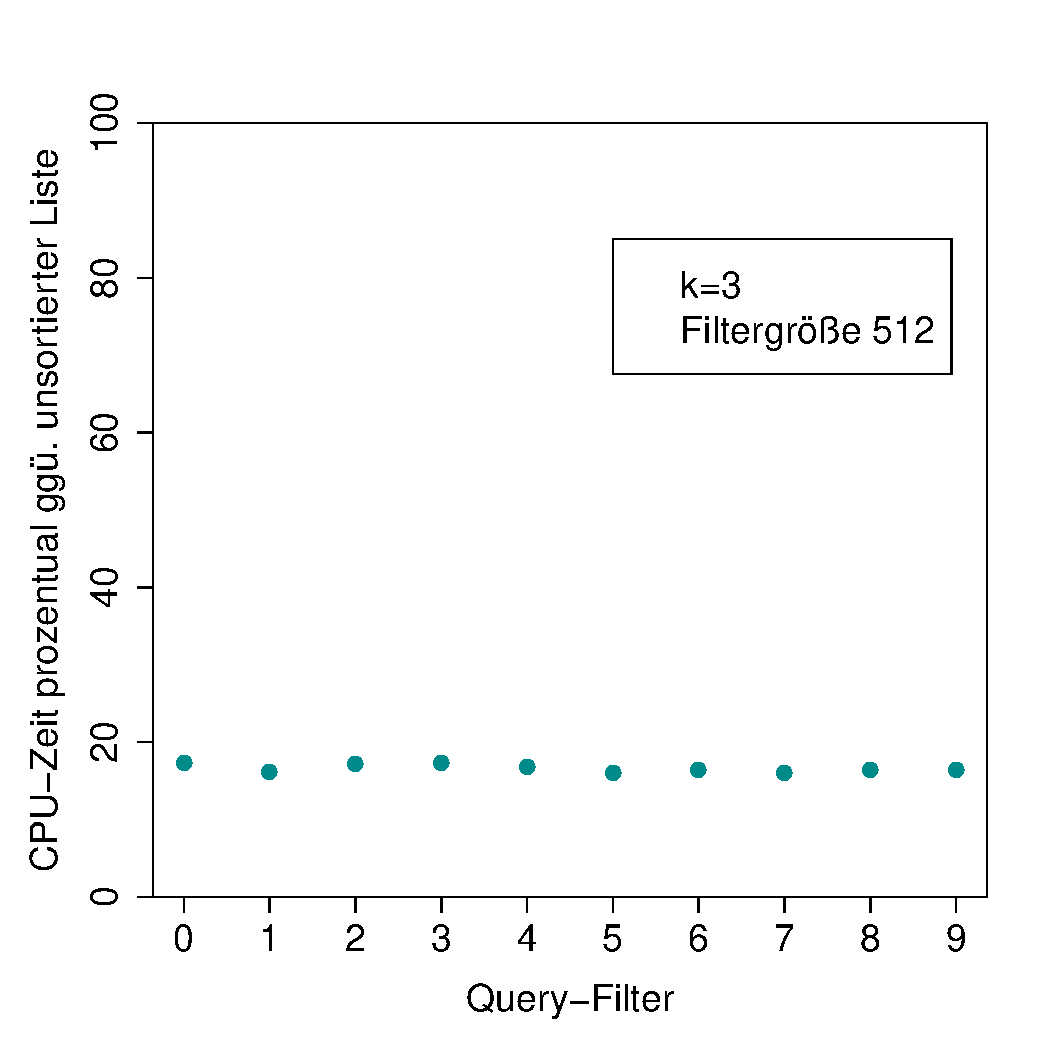
\includegraphics[width=0.48\linewidth]{pictures/percent_time_nn3_512.pdf}}
 \caption[CPU-Zeitersparnis für k-nächste-Nachbarn-Suche im BloomFilterTree]{CPU-Zeitersparnis für k-nächste-Nachbarn-Suche im BloomFilterTree.}
 \label{fig:multipic1} %% label for entire figure
\end{figure}
Daran wird deutlich: Die Zeitersparnis wächst mit dem Parameter \textit{k} und der Filtergröße, doch auch bei $k=1$ wird bereits CPU-Zeit eingespart. Es ist zu erwarten, dass bei größeren BloomFilterTree-Objekten, höheren Anzahlen an Filtern und ggf. größeren Filtern die Zeitersparnis noch deutlich gesteigert werden kann: 

Beim hier verwendeten Versuchsaufbau werden i.d.R Bäume mit drei Ebenen aufgebaut, d.h. bei einer Punktanfrage wird auch bei bestehenden Teil- und Obermengenbeziehungen ein großer Teilbaum durchsucht bzw. ein großer Bereich der Blattebene traversiert. Bei größerer Höhe des Baums durch mehr eingefügte Filter kommen damit die Vorteile des entwickelten Verfahrens deutlicher zum Tragen. Wie in Abbildung \ref{fig:multipic1} erkennbar, gilt ebenso für höhrere Filtergrößen. Die CPU-Zeitersparnis zeigt sich bei Anfragen mit $k>1$ besonders deutlich. Auch hier ist zu erwarten, dass sich die Vorteile des entwickelten Verfahrens bei höheren Bäumen und Filteranzahlen sowie größeren Filtern noch deutlich stärker zeigen.
\newpage
\noindent
Wie in Abschnitt \ref{sec:b+bäume} dargestellt, ist die Komplexität der Suchoperation im B$^+$-Baum abhängig vom Parameter \textit{t}, d.h. dem Grad des Baumes. Die hier verwendeten BloomFilterTree-Objekte haben Grad 3, d.h. die maximale Ausfächerung beträgt 7. Dieser Parameter kann beim Anlegen eines BloomFilterTree-Objekts frei gewählt werden. In der Praxis werden deutlich höhere Werte für t verwendet, z.B. mit 10.000 Elementen pro Knoten beim Einsatz in Datenbank-Managementsystemen. Es ist daher davon auszugehen, dass die Anwendung für ein deutlich größeres Szenario prinzipiell gut geeignet wäre.  
\paragraph*{Speicherbedarf}
Der zusätzliche Speicherbedarf beim BloomFilterTree gegenüber einem Bloom-Filter-Vektor ergibt sich durch die Allokierung eines Vereinigungsfilters für jeden Knoten. Er ist somit abhängig von der Anzahl der Knoten im Baum. Mit dem verwendeten Versuchsaufbau liegt er um 32\% für den BloomFilter gegenüber einem Bloom-Filter-Vektor. Auch hier ließe sich durch eine geringere Knotenanzahl, d.h. BloomFilterTree-Objekte mit höherem Verzweigungsgrad, noch Speicherplatz einsparen. 
\paragraph*{Komplexität}
Auch bezüglich der Zeitkomplexität, d.h. der Abschätzung der notwendigen Berechnungsschritte unabhängig von der gewählten Plattform, zeigt das entwickelte Verfahren erfreuliche Ergebnisse. Die Anzahl der nötigen Vergleiche bei der \textit{k}-nächste-Nachbarn-Suche beträgt 24\% bzw. 32\% beim BloomFilterTree gegenüber der unsortierten Liste. Auch hier ist zu erwarten, dass sich die Ergebnisse bei höheren Bäumen noch verbessern lassen, da bei der \textit{k}-nächste-Nachbarn-Suche nur der beste Pfad verfolgt wird. Bei höheren Bäumen werden somit mehr bzw. größere Teilbäume abgeschnitten und müssen nicht betrachtet werden. 
\paragraph*{Aufbaukosten}
Die Kosten für den Aufbau der Indexstruktur sind erwartungsgemäß ein Wermutstropfen. Auch wenn in der Praxis niedrigere Werte zu erwarten sind, da weniger als \textit{n} freie und "`gute"' IDs sortiert werden müssen, liegen die Aufbaukosten in $O(n\ast log(n))$. Das ist offensichtlich ein starker Zuwachs gegenüber einer unsortierten Liste, die sich z.B. durch ein Objekt vom Typ \texttt{std::vector} realisieren lässt. Andererseits kann davon ausgegangen werden, dass die Aufbaukosten in AMBIENCE deutlich seltener anfallen als z.B. in einem Verteilten System mit häufigem Ausscheiden und Hinzukommen von Knoten wie in den Abschnitten \ref{sec:bloom-netzwerk} und \ref{sec:bloom-index} beschrieben.